\documentclass[../thesis.tex]{subfiles}

\begin{document}

% TODO
% \section{XXX}
% \subsection{xxx}

\section{Dataset}

In order to investigate responsiveness to food in a large scale natural setting, we take advantage of the Natural Scenes Dataset (NSD), a dataset of high-resolution fMRI responses to natural scenes via a recognition task \cite{Allen}. These natural scene images are pulled from the annotated Microsoft Common Objects in Context (COCO) dataset \cite{lin2014microsoft}. NSD has brain response data from 8 screened subjects that each see roughly 9500 natural scene images over the course of a year. These viewings were administered during 30-40 scan sessions. Of the 70,566 total images viewed across participants, 1000 of these images are viewed by all 8 participants. We took special interest in these 1000 images' response data when conducting analysis in order to ensure consistency in results. 


\section{Labeling}

As outlined in Figure 1, we use a categorical hierarchical structure to hand label the 1000 shared images viewed by all subjects with their location classification, object classification (including the binary existence of food), and perspective classification of the image. Image perspective is discretized into 'zoom,' 'reach,' or 'large-scale.' 'zoom' signifies an apparent zoom in of the camera lens, thereby likely focusing on one object and excluding surrounding information. 'reach' images demonstrate affordances by displaying objects at a human-reachable distance \cite{josephs2021world}. 'large-scale' images encompass the remaining images, which likely include an image of a general scene as opposed to one or more close up objects. The image perspective category's vague nature leaves it vulnerable to variation in labeling. To avoid this variation and ensure consistency, we underwent several rounds of labeling and verification. 

\begin{figure}
    \centering
    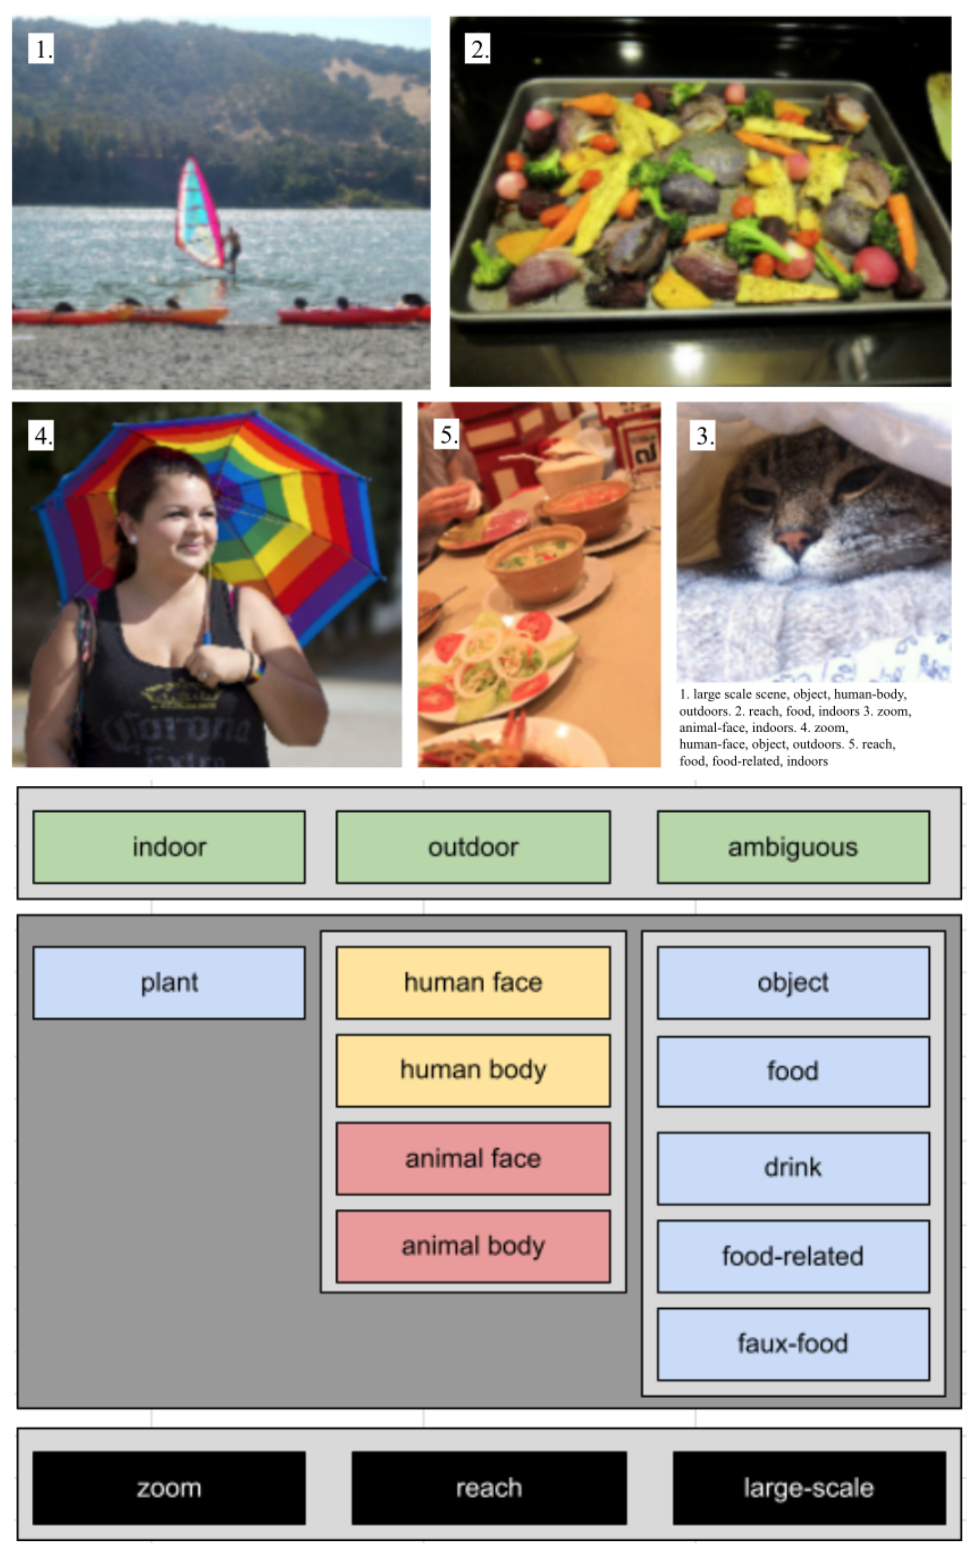
\includegraphics[scale=0.6]{fig1.png}
        \caption{The 1000 images viewed by all 8 subjects in NSD were manually relabeled in order to investigate responsiveness to natural food images. The top half of this figure shows example images that were labeled as well as their corresponding labels, while the bottom half demonstrates the organizational structure used when labeling a given image. Each of the images were given at least one label within each of the three categories of location, content, and image perspective. Multiple content labels could be and often were used for a given image} \label{fig1}
\end{figure}

\section{Encoding and Decoding models}
To identify voxels especially responsive to certain labels, we encode all 16 labels into a single binary vector per image and perform voxel-wise ordinary least squares encoding models. We then run statistical significance tests between pairs of weights, where each weight is the model coefficient for a different label input. 

While an encoding model is able to provide some insight into single-voxel selectivity through response predictions, a decoding model can uncover distributed pattern-level representations of visual features. As a result, we perform a voxel-wise searchlight algorithm to classify the existence of food and further inspect high-performing regions. 

\section{Understanding fine grained region structure}
Encoding and decoding models help identify proposed regions especially responsive to food, but are unable to provide further insight regarding the structure of these 'food regions'. We run a principal component analysis to better understand the structure and correspondence in these food regions. To verify our proposed food regions resulting from analysis on the 1000 shared images, we perform further investigation across the remaining images that were not already used. These remaining images are no longer hand labeled, so we use we use a ridge regression model on COCO labels and visualized the resulting voxel-wise weights per label. \\

In addition to investigating the weights of the ridge regression, we directly consider the non-shared images' activation patterns in our proposed food region. Using the proposed region as a voxel mask, we extract each image's corresponding food-voxel activity. We then perform a K-means clustering algorithm on this activity and investigate the resulting groups. In order to better understand potential visual and semantic justifications behind these voxel-based clusters and isolate these justifications from top-down cortical influences, we also cluster visual and semantic embeddings of these images and look for possible correlations between the image clustering results and voxel clustering results. To obtain these visual and semantic embeddings we use two state of the art models, CLIP and ResNet-50 \cite{radford2021learning, he2016deep}. CLIP, trained on both images and text, allows us to extract features with semantic and visual meaning. ResNet-50, training on solely images, results in purely visual feature-based embeddings. 



\end{document}